
\section{Methodik}
\subsection{Datenaufbereitungsprozess}
Die Vorbereitung der Daten beginnt mit den Basisinformationen zu Quadratmeterpreisen. Es wird ein Datensatz generiert, der drei Anforderungen erfüllt. Erstens: Die Wohnfläche für Eigenheime liegt zwischen 80 und 200 Quadratmetern. Zweitens: Die LTV-Verteilung ähnelt der der Münchener Hypothekenbank mit einem Durchschnitt von etwa 60\%. Drittens: Der durchschnittliche Darlehensbetrag nähert sich 163.700 € an. Alle Werte werden gemäß Berechnungsformeln ermittelt:
\begin{equation}
    \text{Immobilienwert} = \text{Quadratmeterpreis} \cdot \text{Wohnfläche}
\end{equation}
\begin{equation}
    \text{Darlehensbetrag} = \text{Immobilienwert} \cdot \text{aktuelles\_LtV}
\end{equation}
Abbildung \ref{fig:flowchart} visualisiert diesen Datenaufbereitungsprozess. Der Datenaufbereitungsprozess beginnt mit dem Einlesen einer CSV-Datei, die bereits Immobilien-IDs, Geometriedaten, Überschwemmungsrisikoinformationen, Energieklassen und Quadratmeterpreise enthält. Anschließend wird eine Spalte \enquote{wohnflaeche} erstellt, gefolgt von der Generierung einer Spalte \enquote{aktuelles\_LtV}. Der nächste Schritt beinhaltet die Berechnung des \enquote{aktuellen\_Immobilienwerts}. Ein kritischer Entscheidungspunkt folgt, bei dem geprüft wird, ob der LtV-Mittelwert kleiner als 60\% ist. Falls ja, werden die LtV-Werte angepasst. Andernfalls wird ohne Anpassung fortgefahren. Danach wird die Spalte \enquote{Darlehensbetrag} berechnet.

Der zweite Entscheidungspunkt überprüft, ob der Darlehensbetrag-Mittelwert gleich 163.700 € ist. Wenn nicht, wird die Wohnfläche angepasst und eine Neuberechnung von \enquote{aktuellen\_Immobilienwert} und \enquote{Darlehensbetrag} durchgeführt. Bei Erfüllung der Bedingung wird der Prozess ohne Änderungen fortgesetzt. Die letzten Schritte umfassen die Überprüfung der Formeln, das Speichern der Ergebnisse in einer neuen CSV-Datei und abschließend die Prüfung des endgültigen Mittelwerts des Darlehensbetrags. Dieser strukturierte Ablauf gewährleistet eine präzise und konsistente Datenaufbereitung für die Immobilienbewertung.

\begin{figure}[H]
    \centering
    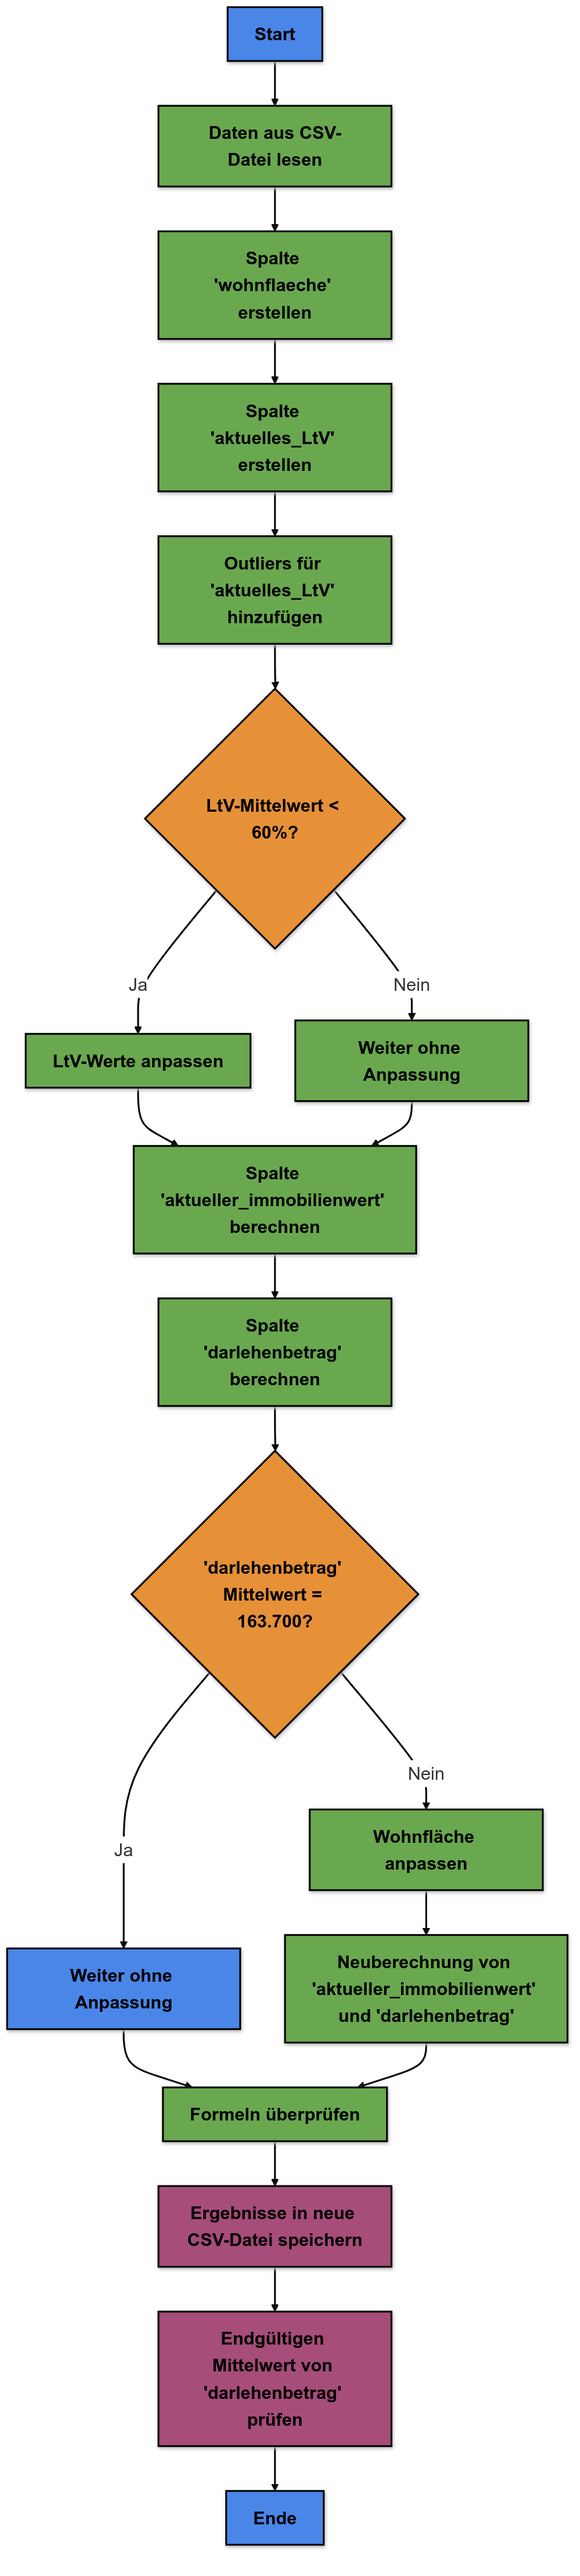
\includegraphics[width=0.3\textwidth]{figures/flowchardatatensatz.png}
    \caption{Prozessablauf Immobilienwertberechnung. Quelle: Eigene Darstellung}
    \label{fig:flowchart}
\end{figure}

\subsection{Quantifizierung physischer Risiken}
In diesem Abschnitt wird bei der Modellierung des Hochwasserrisikos die grundlegende Quantifizierung des physischen Risikos erläutert.

\subsubsection{Schadensfunktion}\label{sec:schadenfkt}
Wie bereits in Abschnitt \ref{sec:tief} erwähnt, hängen die Schäden durch Überschwemmungen von der Wassertiefe ab. In diesem Abschnitt wird erklärt, wie diese Abhängigkeit konkret besteht.
Sobald verschiedene Flutwassertiefen ermittelt sind, wird eine spezifische Schadensfunktion für Wohnimmobilien \acs{RRE} entwickelt. Diese basiert auf der Methodik des Gemeinsamen Forschungszentrums \acs{JRC} der Europäischen Union \parencite{huizinga2017global}.

Allerdings ist die Datengrundlage für diese Analyse begrenzt, da das veröffentlichte \acs{JRC}-Dokument keine spezifische Schadensfunktion für Wohngebäude bereitstellt und die zugrunde liegende Studie von \textcite{huizinga2007flood} nicht publiziert wurde. Folglich müssen die erforderlichen Informationen aus den verfügbaren Diagrammen extrahiert werden.

Abbildung \ref{fig:damage_curve1} und \ref{fig:damage_curve2} präsentieren zwei Grafiken, die die Schadenshöhe pro Quadratmeter und den Schadensfaktor für unterschiedliche europäische Regionen veranschaulichen.

\begin{figure}[H]
    \centering
    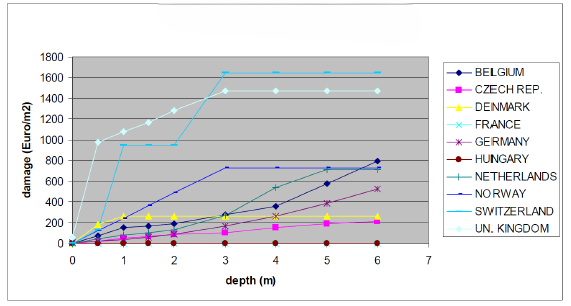
\includegraphics[width=0.8\textwidth]{figures/RREdamagem2.png}
    \caption{Schaden pro Quadratmeter in verschiedenen Regionen Europas. Quelle: J. Huizinga und al., 2017}
    \label{fig:damage_curve1}
\end{figure}

\begin{figure}[H]
    \centering
    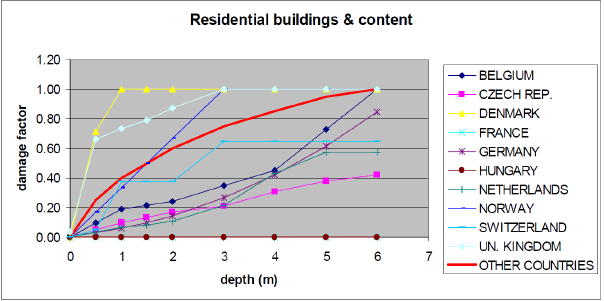
\includegraphics[width=0.8\textwidth]{figures/RREdamage.png}
    \caption{Schadensfaktor für Wohnimmobilien in verschiedenen Regionen Europas. Quelle: J. Huizinga und al., 2017}
    \label{fig:damage_curve2}
\end{figure}

\subsubsection{Risikogewichte}
Basel III ist ein globales Regelwerk, das nach der Finanzkrise 2008 zur Stabilisierung des Bankensektors eingeführt wurde. Der Abschnitt \acs{CRE}20 beschreibt die Vorgaben zur Berechnung der \ac{RWA}, wobei feste Risikogewichte für verschiedene Kreditarten vorgeschrieben werden. Für Wohnimmobilienkredite, die nicht vom durch die Immobilie generierten Cashflow abhängen, werden die Risikogewichte anhand des \ac{LtV}-Verhältnisses bestimmt: Je höher der \ac{LtV}, desto höher das Risikogewicht.

\begin{table}[htbp]
    \centering
    \caption{Risikogewichte basierend auf dem LtV-Verhältnis für Wohnimmobilienkredite. Quelle: Vanweddingen, 2023 }
    \label{tab:rwa_ltv}
    \small 
    \begin{tabularx}{\textwidth}{>{\raggedright\arraybackslash}X*{6}{>{\centering\arraybackslash}X}} 
    \toprule
    \textbf{LtV} & $\leq 50\%$ & $50$--$60\%$ & $60$--$80\%$ & $80$--$90\%$ & $90$--$100\%$ & $>100\%$ \\
    \cmidrule(lr){1-7} 
    \textbf{Risikogewicht} & 20\% & 25\% & 30\% & 40\% & 50\% & 70\% \\
    \bottomrule
    \end{tabularx}
\end{table}




In Tabelle \ref{tab:rwa_ltv} wird das Risikogewicht in Abhängigkeit vom \ac{LtV}-Verhältnis dargestellt.

\subsubsection{Berechnung von Immobilienwerten unter Hochwasserrisiko}
Gemäß der Definition von der \textcite{undro1979} ergibt sich das Risiko aus drei Komponenten: Gefährdungswahrscheinlichkeit,  den betroffenen Elemente (Exposition) und Vulnerabilität. \parencite{coburn1991vulnerability}. Dies kann vereinfacht ausgedrückt werden als:

\begin{equation}
    \text{Physisches Risiko} = \text{Gefährdungswahrscheinlichkeit} \times \text{Exposition} \times \text{Vulnerabilität}
\end{equation}

Um eine genauere Analyse der einzelnen Immobilienschäden zu ermöglichen, wird eine detailliertere Schadensformel \parencite{vanweddingen2023physicalrisk} benutzt:
\begin{equation}
    Immobilienschaden_{i,j} = E_j \times d(I_{i,j}|v_j)
    \label{eq:schaden}
\end{equation}
Wobei:
\begin{itemize}
    \item i das spezifische Ereignis bezeichnet
    \item $E_j$ den Wert der einzelnen Immobilie am Standort j repräsentiert
    \item $d$ die spezifische Schadensfunktion darstellt
    \item $I_{i,j}$ die lokale Intensität des Ereignisses i am Standort j ist
    \item $v_j$ die spezifische Vulnerabilität der einzelnen Immobilie am Standort j bezeichnet
\end{itemize}

Formel \ref{eq:schaden} berücksichtigt die Gefährdungswahrscheinlichkeit nicht, da sie den Schaden für ein einzelnes Ereignis berechnet. Für den erwarteten jährlichen Immobilienschaden wird die jährliche Überschreitungswahrscheinlichkeit aus Kapitel \ref{sec:EPC} benötigt und wird nachfolgend berechnet:
\begin{equation}
    EAI_j = \sum_i Immobilienschaden_{i,j} \times p(I_{i,j})
    \label{eq:EAI}
\end{equation}
Hierbei steht \acs{EAI} für den erwarteten jährlichen Schaden, und \( p(I_{i,j}) \) ist die Eintrittswahrscheinlichkeit des Ereignisses \( i \) mit der Intensität \( I_{i,j} \) am Standort \( j \).

Die Auswirkungen auf den Immobilienwert nach einem Schaden werden wie folgt berechnet:
\begin{equation}
    \text{Neuer Immobilienwert} = \text{Ursprünglicher Immobilienwert} - \text{Schaden}
\end{equation}

Zur Bestimmung der neuen Beleihungsquote \ac{LtV} auf Basis des angepassten Immobilienwertes gilt:
\begin{equation}
    \text{Neue LtV} = \frac{\text{Darlehenbetrag}}{\text{Neuer Immobilienwert}}
\end{equation}

Die risikogewichteten Aktiva \acs{RWA}, abhängig von der Beleihungsquote, berechnen sich folgendermaßen:
\begin{equation}
    RWA = \text{Darlehenbetrag} \times \text{Risikogewicht}
\end{equation}
Das Risikogewicht wird anhand der Beleihungsquote ermittelt.

Zum Schluss lässt sich die prozentuale Änderung der \acs{RWA} mit dieser Formel bestimmen:
\begin{equation}
    \% \text{Änderung RWA} = \frac{\text{Neue RWA}}{\text{Ursprüngliche RWA}} - 1
\end{equation}
\subsection{Quantifizierung von Transitionsrisiken}
\subsubsection{Berechnung der Endenergiepreise}
Die \ac{NGFS}-Szenarien und die zugehörige Modellierung der Energiepreise sind wesentlich für eine Bewertung von Immobilien. Die beschriebenen Szenarien im Abschnitt \ref{sec:ngfs} beinhalten verschiedene Entwicklungsmöglichkeiten der Energiepreise.

Die Energiepreise basieren auf einer Kombination aus Öl- und Gaspreisen, die den Hauptanteil des Energieverbrauchs in deutschen Wohngebäuden ausmachen. Die Heizenergiepreis von 5,89~\text{Cent/kWh} im Jahr 2020 in Deutschland \parencite{behr2023warmemonitor} dient als Referenzpunkt für die Preisentwicklung in den verschiedenen Szenarien. Darüber hinaus müssen CO\textsubscript{2}-Steuern in die Betrachtung der zukünftigen Energiekosten einbezogen werden. Die Berechnung der Energiepreise folgt der von \textcite{tergerman} beschriebenen Methodik mit einer erweiterten Formel für den Endpreis:
\begin{equation}\label{eq:pt}
P_t = (1 + \tau_t) \cdot [\omega^O \cdot (\frac{\kappa^O \cdot T^{CO2}_t}{1000} + \frac{P^O_t}{E_t \cdot \gamma}) + (1 - \omega^O) \cdot (\frac{\kappa^G \cdot T^{CO2}_t}{1000} + \frac{P^G_t}{E_t \cdot \gamma})]
\end{equation}
Hierbei ist $P_t$ der Endpreis der Energie, $\tau_t$ die Mehrwertsteuer, $\omega^O$ der Anteil von Öl am Energiemix (35\%), $P^O_t$ und $P^G_t$ die Rohstoffpreise von Öl und Gas in Dollar, $T^{CO2}_t$ die CO\textsubscript{2}-Steuer, $E_t$ der Wechselkurs Dollar/Euro, $\kappa^O$ und $\kappa^G$ die CO\textsubscript{2}-Emissionsfaktoren für Öl und Gas, und $\gamma$ der Umrechnungsfaktor von Barrel Öläquivalent zu kWh. Wichtige Konstanten aus dem Anhang B [S. 15] sind: $\kappa^O = 0,287$ kg CO\textsubscript{2}/kWh für Öl, $\kappa^G = 0,238$ kg CO\textsubscript{2}/kWh für Gas, und $\gamma = 1700$ kWh/BOE \parencite{tergerman}. 

Die Daten für $P^O_t$, $P^G_t$ und $T^{CO2}_t$ entstammen den im Abschnitt \ref{sec:ngfs_preis} beschriebenen Datenquellen.
Abbildung \ref{fig:endpreis_energie} zeigt das Resultat der Gleichung \ref{eq:pt} bezüglich des Endpreises für Energie, unter Berücksichtigung der Mehrwert- und Energiesteuern gemäß den NGFS-Szenarien.

\begin{figure}[htbp]
    \centering
    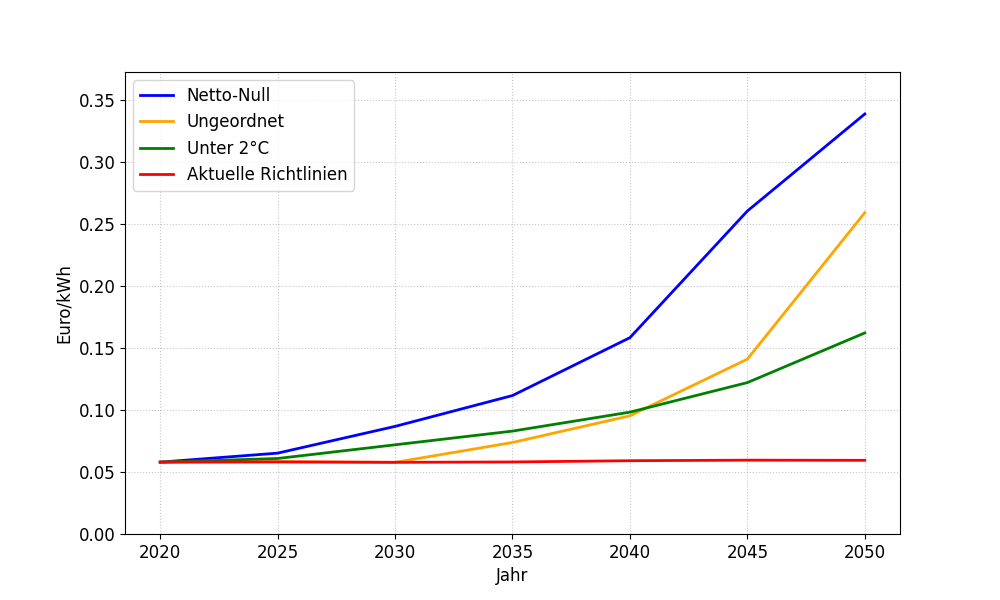
\includegraphics[width=\textwidth]{figures/endpreis.png}
    \caption{Endpreis der Energie mit Mehrwert- und CO2-Steuern nach NGFS-Szenarien. Quelle: Eigene Darstellung}
    \label{fig:endpreis_energie}
\end{figure}
\FloatBarrier
\subsubsection{Berechnung von Immobilienwerten unter Energiepreisänderungen}
Nach der Modellierung der Energiepreise gemäß NGFS-Szenarien und deren zeitlicher Entwicklung wird im Folgenden die konkrete Anwendung dieser Daten für die Immobilienbewertung erläutert.

Die Studie von \parencite{tergerman} bietet einen Ansatz zur Quantifizierung der Auswirkungen von Energiepreisänderungen auf Immobilienwerte. Die Kerngleichung lautet:

\begin{equation}
D^j_t(S) \equiv \frac{P^j_t(S) - P^{A+}_t(S)}{P^{A+}_t(S)} = -\frac{P^E_t \Delta EE^j}{P^{A+}_t(S)} \sum_{h=1}^T \frac{g^E_{t+h}(S)}{(1 + r)^h}
\end{equation}
Wobei:
\begin{itemize}
    \item $D^j_t(S)$: Der relative Preisabschlag einer Immobilie mit Energieeffizienzklasse $j$ zum Zeitpunkt $t$ im Szenario $S$.
    \item $P^j_t(S)$: Der Preis einer Immobilie der Energieeffizienzklasse $j$ zum Zeitpunkt $t$ im Szenario $S$.
    \item $P^{A+}_t(S)$: Der Preis einer Immobilie der höchsten Energieeffizienzklasse A+ zum Zeitpunkt $t$ im Szenario $S$.
    \item $P^E_t$: Der Energiepreis zum Zeitpunkt $t$.
    \item $\Delta EE^j$: Die Energieeffizienzdifferenz zwischen der Immobilie der Klasse $j$ und der Klasse A+.
    \item $g^E_{t+h}(S)$: Der Wachstumsfaktor des Energiepreises zum Zeitpunkt $t+h$ im Szenario $S$.
    \item $r$: Die Diskontierungsrate.
    \item $T$: Der betrachtete Zeitraum.
\end{itemize}
Für die Bewertung einzelner Immobilien wurde diese Gleichung wie folgt adaptiert:

\begin{equation}
    \Delta EC_{rel} = (E_j - E_{A+}) \cdot (PE_1 - PE_0) \cdot A
    \end{equation}
    \begin{equation}
    \Delta P = -\Delta EC_{rel} \cdot \frac{1 - (1 + r)^{-T}}{r}
    \end{equation}
    In dieser angepassten Form beschreibt $\Delta P$ die absolute Wertänderung der Immobilie, basierend auf der relativen Änderung der Energiekosten $\Delta EC_{rel}$. Diese berücksichtigt die Differenz im Energieverbrauch $(E_j - E_{A+})$, die Energiepreisentwicklung $(PE_1 - PE_0)$ sowie die Fläche der Immobilie $A$.
    Anschließend wird die prozentuale Wertänderung ermittelt:
    \begin{equation}
    D_t = \frac{\Delta P}{P_0}
    \end{equation}
    Basierend auf diesen Berechnungen lässt sich der neue Wert des Gebäudes bestimmen:
    \begin{equation}
    \text{Neuer Immobilienwert} = P_0 + \Delta P
    \end{equation}
    Schließlich kann der aktualisierte \ac{LtV} berechnet werden:
    \begin{equation}
    \text{Neuer LtV} = \frac{\text{Darlehenbetrag}}{\text{Neuer Immobilienwert}}
    \end{equation}

Diese zweistufige Methodik ermöglicht eine differenzierte Analyse der Wertveränderungen unter Berücksichtigung unter energiepreisbedingter Einflüsse sowie eine Neubewertung des Beleihungsauslaufs.